\graphicspath{{Chapter3/Section3.3/Figs/}}


\begin{table}[tb]
  \caption{Prediction performance of reference model and the proposed model over subjective experiment}
  \centering
  \begin{tabular}{|c|c|c|c|c|}
    \hline
    & PCC & SROCC & RMSE & OR (\%)\\
    \hline
    \cite{CumulativeQoE_Assessing} & \textbf{0.5418} & 0.3917 & 9.1318 & 33.3\\ \hline
    Proposed model & 0.5405 & \textbf{0.5146} & \textbf{9.0922} & \textbf{25.0}\\
    \hline
  \end{tabular}
  \label{tbl:PerformanceExperiment}
\end{table}


\begin{figure}[tb]
  \centering
  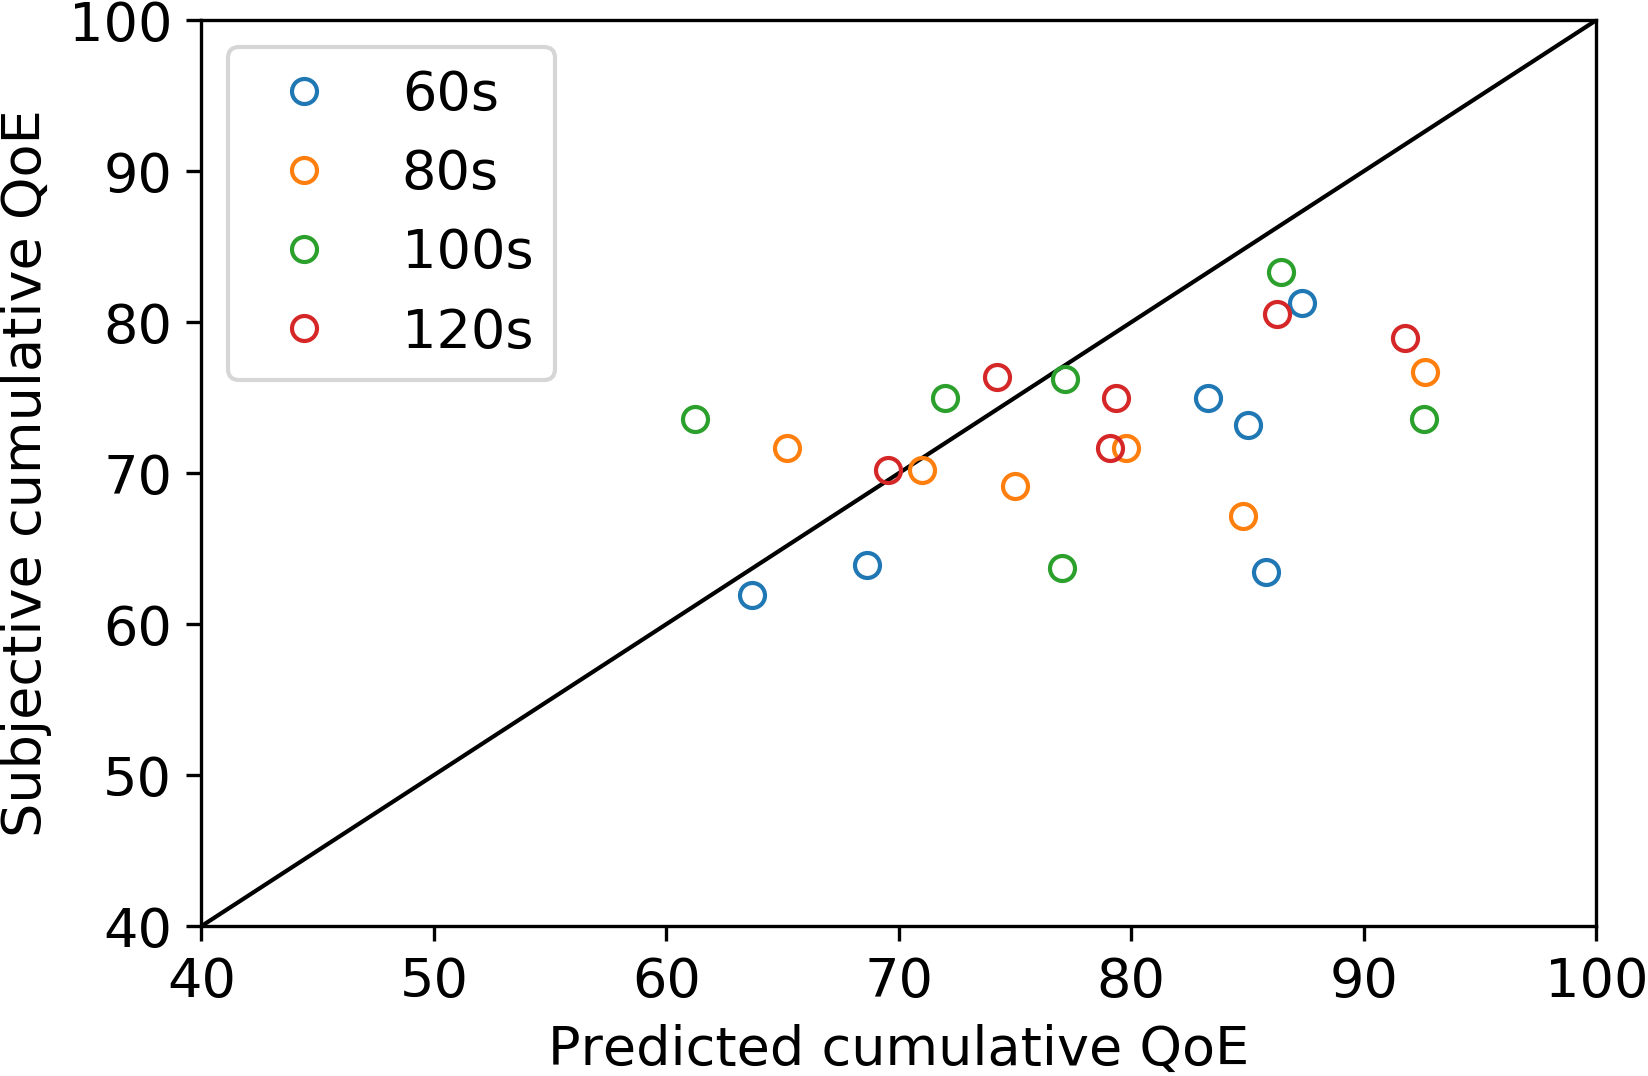
\includegraphics[width=0.5\linewidth]{\FigsDir/pcc_cmqoe_mosqoe.png}
  \caption{Scatter plot of predicted cumulative QoE and subjective cumulative QoE.}
  \label{fig:PCC_CumulativeQoE_MOSQoE}
\end{figure}

\begin{figure}[tb]
  \centering
  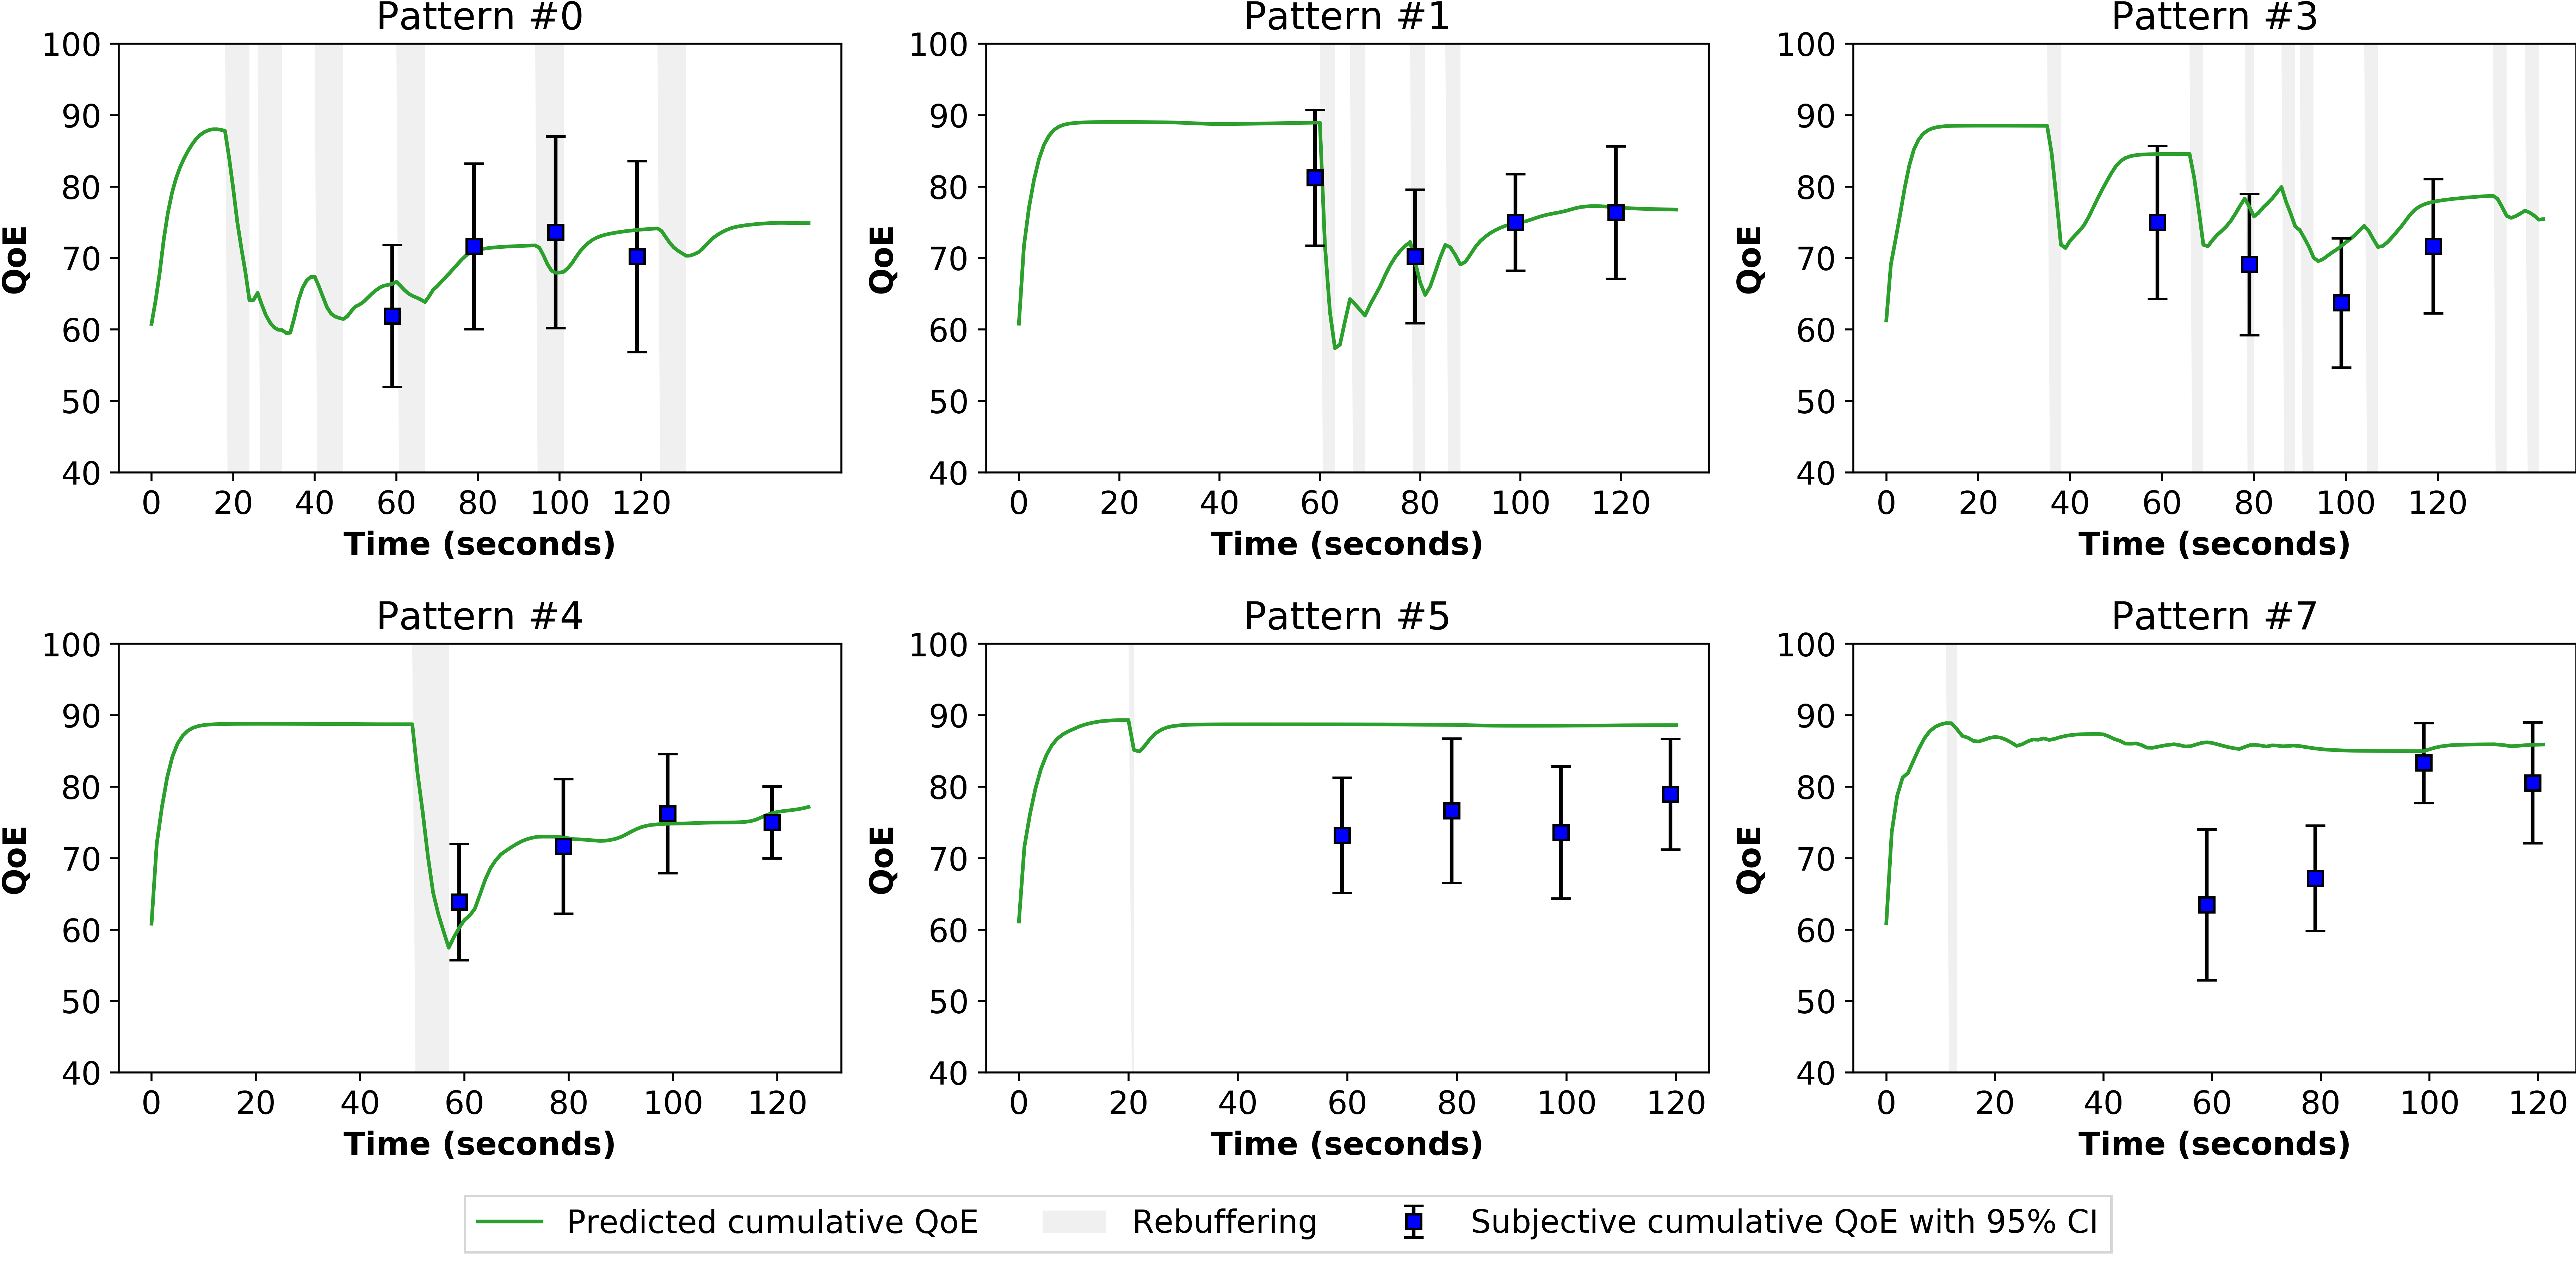
\includegraphics[width=\linewidth]{\FigsDir/cumulative_performance_experiment.png}
  \caption{Performance of our predicted cumulative QoE in comparison with the subjective cumulative QoE.}
  \label{fig:CumulativePerformanceExperiment}
\end{figure}

In this subsection, a subjective evaluation is conducted to assess the accuracy of the proposed model aligning with ground truth QoE scores provided by a number of subjects. The performance of QoE prediction using the proposed model is evaluated by relying on the following four measures: 1) PCC, 2) SROCC, 3) RMSE and 4) Outage Rate (OR) \cite{QoEModel_TimeVaryingSubjectiveQuality}. While PCC and SROCC quantify the correlation between predicted cumulative QoE and the subjective cumulative QoE, the closeness between predicted scores and the ground truth scores is numerically obtained by using RMSE and OR. In particular, OR measures the frequency of times when the prediction $p_{i}$ falls outside twice the confidence interval of subjective scores $s_{i}$, which is defined as the following equation:
\begin{equation}
    OR = \frac{1}{N}\sum^{N}_{i}{\mathbbm{1}(\left | p_{i} - s_{i} \right | > 2CI_{s_{i}} )}
\end{equation}
where $\mathbbm{1}$($\cdot$) is the indicator function

To conduct the subjective test, 6 distorted videos from the testing set of LFOVIA database (pattern \#0, \#1, \#3, \#4, \#5, \#7) were selected. We selected those videos because they have different contents, thus, the role of DoI in our model can be potentially assessed. Each distorted video was cropped into 4 small videos with starting timestamps of 00:00:00 and different length (60, 80, 100, and 120 seconds) using FFmpeg \cite{FFmpeg}. The purpose is to ask the subjects to provide subjective cumulative evaluations at the time points of 60, 80, 100, and 120 seconds of each distorted video. The correlations between subjective cumulative QoE and predicted cumulative QoE obtained from our model and reference model were assessed. The cropped videos were divided into 6 collections with different video content and displayed on a 15-inch screen with a resolution of 1920x1080 and a black background. Each video was rated by at least 18 subjects and there were totally 120 participants. Note that these subjects are different from those in "DoI" experiment in subsection 3.3. The Absolute Category Rating method was used in our experiment \cite{ITUT_P913}. The subjects give a rating score at the end of each cropped video with the score ranging from 1 (worst) to 5 (best) based on the perceived quality and video content, following the general principle of the ITU-T recommendation P.913 \cite{ITUT_P913}. The average of subjects scores, associated with 95\% confidence interval, for each cropped video, was utilized as the subjective cumulative QoE. These values were linearly rescaled so that the scores lay in the range [0, 100] and then compared with the predicted cumulative QoE.

Figure \ref{fig:PCC_CumulativeQoE_MOSQoE} illustrates the obtained correlation between the predicted cumulative QoE and subjective cumulative QoE. The comparison in QoE prediction performance between our model and reference model is tabulated in Table \ref{tbl:PerformanceExperiment}. Accordingly, we observe that the proposed model provides a competitive performance in terms of SROCC, RMSE and OR against the reference model. On the other hand, Fig. \ref{fig:CumulativePerformanceExperiment} shows a reasonable prediction performance of our model in comparison with subjective cumulative QoE at four discrete moments (at time points of 60, 80, 100, and 120 seconds) within a streaming session. In general, the proposed model performs extremely well when the high frequent and long duration rebuffering occur. It means that our model is capable of cumulatively capturing the effects of all the occurred unpleasant events on human perception. However, the model performance in pattern \#5 and \#7 are poorer, as compared to other patterns (\#0, \#1, \#4) even though they have only one short rebuffering event. This can be explained that in pattern \#5 and \#7, the users' perception seems to be significantly affected by the video content. In other words, the effect of DoI become dominant in their evaluation, which is not precisely captured by our model.
